%++++++++++++++++++++++++++++++++++++++++
\documentclass[article, 12pt]{article}
\usepackage{float}
\usepackage{setspace}
\usepackage{tabu} % extra features for tabular environment
\usepackage{amsmath}  % improve math presentation
\usepackage{graphicx} % takes care of graphic including machinery
\usepackage[margin=1in]{geometry} % decreases margins
\usepackage{cite} % takes care of citations
\usepackage[final]{hyperref} % adds hyper links inside the generated pdf file
\usepackage{tikz}
\usepackage{caption} 
\usepackage{fancyhdr}
\usepackage{amssymb} % symbols like /therefore
\usepackage{amsthm} % proofs
\usepackage{enumerate} % lettered lists
\usepackage{mathtools} % macros
\usepackage{stix}
\usetikzlibrary{scopes}
% \usepackage{xcolor} \pagecolor[rgb]{0.12549019607,0.1294117647,0.13725490196} \color[rgb]{0.82352941176,0.76862745098,0.62745098039} % dark theme
\theoremstyle{definition}
\newtheorem{example}{Example}[subsubsection]
\newtheorem*{remark}{Remark}
\newtheorem{theorem}{Theorem}[subsubsection]
\newtheorem{definition}{Definition}[subsubsection]
\newtheorem{corollary}{Corollary}[subsubsection]
\hypersetup{
	colorlinks=false,      % false: boxed links; true: colored links
	linkcolor=blue,        % color of internal links
	citecolor=blue,        % color of links to bibliography
	filecolor=magenta,     % color of file links
	urlcolor=blue         
}
\usepackage{physics}
\usepackage{siunitx}
\usepackage{tikz,pgfplots}
\usepackage[outline]{contour} % glow around text
\usetikzlibrary{calc}
\usetikzlibrary{angles,quotes} % for pic
\usetikzlibrary{arrows.meta}
\tikzset{>=latex} % for LaTeX arrow head
\contourlength{1.2pt}

\colorlet{xcol}{blue!70!black}
\colorlet{vcol}{green!60!black}
\colorlet{myred}{red!70!black}
\colorlet{myblue}{blue!70!black}
\colorlet{mygreen}{green!70!black}
\colorlet{mydarkred}{myred!70!black}
\colorlet{mydarkblue}{myblue!60!black}
\colorlet{mydarkgreen}{mygreen!60!black}
\colorlet{acol}{red!50!blue!80!black!80}
\tikzstyle{CM}=[red!40!black,fill=red!80!black!80]
\tikzstyle{xline}=[xcol,thick,smooth]
\tikzstyle{mass}=[line width=0.6,red!30!black,fill=red!40!black!10,rounded corners=1,
                  top color=red!40!black!20,bottom color=red!40!black!10,shading angle=20]
\tikzstyle{faded mass}=[dashed,line width=0.1,red!30!black!40,fill=red!40!black!10,rounded corners=1,
                        top color=red!40!black!10,bottom color=red!40!black!10,shading angle=20]
\tikzstyle{rope}=[brown!70!black,very thick,line cap=round]
\def\rope#1{ \draw[black,line width=1.4] #1; \draw[rope,line width=1.1] #1; }
\tikzstyle{force}=[->,myred,very thick,line cap=round]
\tikzstyle{velocity}=[->,vcol,very thick,line cap=round]
\tikzstyle{Fproj}=[force,myred!40]
\tikzstyle{myarr}=[-{Latex[length=3,width=2]},thin]
\def\tick#1#2{\draw[thick] (#1)++(#2:0.12) --++ (#2-180:0.24)}
\DeclareMathOperator{\sn}{sn}
\DeclareMathOperator{\cn}{cn}
\DeclareMathOperator{\dn}{dn}
\def\N{80} % number of samples in plots


\usepackage{titling}
\renewcommand\maketitlehooka{\null\mbox{}\vfill}
\renewcommand\maketitlehookd{\vfill\null}
\usepackage{siunitx} % units
\usepackage{verbatim} 
\newcommand{\courseNumber}{MATH 263}
\newcommand{\courseName}{Discrete Mathematics 2}
\newcommand{\professor}{Dr. Petrescu}
\newcommand{\psetName}{Practice Exam 1}
\newcommand{\dueDate}{Due: February 6, 2023}
\newcommand{\name}{Denny Cao}
\pagestyle{fancy}
\fancyhf{}% clears all header and footer fields
\fancyfoot[C]{--~\thepage~--}
\renewcommand*{\headrulewidth}{0.4pt}
\renewcommand*{\footrulewidth}{0pt}
\lhead{\name}
\chead{\courseNumber: \courseName}
\rhead{\professor}
\newcounter{questionNumber}
\newcommand{\question}[1]{\stepcounter{questionNumber}\noindent\textbf{Problem \arabic{questionNumber}:} #1}
\newcommand{\answer}[1]{\noindent\textbf{Answer:} #1}

\fancypagestyle{plain}{%
  \fancyhf{}% clears all header and footer fields
  \fancyfoot[C]{--~\thepage~--}%
  \renewcommand*{\headrulewidth}{0pt}%
  \renewcommand*{\footrulewidth}{0pt}%
}

% Shortcuts
\DeclarePairedDelimiter\ceil{\lceil}{\rceil} % ceil function
\DeclarePairedDelimiter\floor{\lfloor}{\rfloor} % floor function

\DeclarePairedDelimiter\paren{(}{)} % parenthesis

\newcommand{\df}{\displaystyle\frac} % displaystyle fraction
\newcommand{\qeq}{\overset{?}{=}} % questionable equality

\newcommand{\Mod}[1]{\;\mathrm{mod}\; #1} % modulo operator

\newcommand{\comp}{\circ} % composition

% Sets
\DeclarePairedDelimiter\set{\{}{\}}
\newcommand{\unite}{\cup}
\newcommand{\inter}{\cap}

\newcommand{\reals}{\mathbb{R}} % real numbers: textbook is Z^+ and 0
\newcommand{\ints}{\mathbb{Z}}
\newcommand{\nats}{\mathbb{N}}
\newcommand{\rats}{\mathbb{Q}}

\newcommand{\degree}{^\circ}

% Counting
\newcommand\perm[2][^n]{\prescript{#1\mkern-2.5mu}{}P_{#2}}
\newcommand\comb[2][^n]{\prescript{#1\mkern-0.5mu}{}C_{#2}}

% Relations
\newcommand{\rel}{\mathcal{R}} % relation
\setlength\parindent{0pt}

% Directed Graphs
\usetikzlibrary{arrows}
\tikzset{vertex/.style = {shape=circle,draw,minimum size=1.5em}}
\tikzset{edge/.style = {->,> = latex'}}

% Sign Charts
\newdimen\tcolw \tcolw=2.5em % the column width
\edef\ecatcode{\catcode`&=\the\catcode`&\relax}\catcode`&=4
\def\sgchart#1#2{\vbox{\offinterlineskip\halign{\hfil##\quad&##\hfil\crcr\sgchartA#2,:,%
   \omit\sgchartR&\kern.2pt\sgchartS{.5\tcolw}\relax\sgchartE#1,\relax,%
   \sgchartS{.5\tcolw}\relax\cr
   \noalign{\kern2pt}&\def~{}\kern.5\tcolw\sgchartD#1,\relax,\cr}}}
\def\sgchartA#1:#2,{\cr\ifx,#1,\else $#1$&\sgchartB#2{}\expandafter\sgchartA\fi}
\def\sgchartB#1{\hbox to\tcolw{\hss$#1$\hss}\sgchartC}
\def\sgchartC#1{\ifx,#1,\else
   \strut\vrule\kern-.4pt\hbox to\tcolw{\hss$#1$\hss}\expandafter\sgchartC\fi}
\def\sgchartD#1#2,{\ifx\relax#1\else\hbox to\tcolw{\hss$#1#2$\hss}\expandafter\sgchartD\fi}
\def\sgchartE#1#2,{\ifx\relax#1\else
    \ifx~#1\sgchartS\tcolw\circ \else\sgchartS\tcolw\bullet\fi \expandafter\sgchartE\fi}
\def\sgchartR{\leaders\vrule height2.8pt depth-2.4pt\hfil}
\def\sgchartS#1#2{\hbox to#1{\kern-.2pt\sgchartR \ifx\relax#2\else
   \kern-.7pt$#2$\kern-.7pt\sgchartR\fi\kern-.2pt}}
\ecatcode
%++++++++++++++++++++++++++++++++++++++++
\title{
    \vspace{2in}
    \textmd{\textbf{\courseNumber: \courseName}}
    \normalsize\vspace{0.1in}\\
    \vspace{0.1in}\Large{\text{\psetName}} \\
    \vspace{0.1in}\large{\text{\professor}}
    \vspace{3in}
}

\author{\name}
\date{\dueDate}

\begin{document}
    \maketitle
    \thispagestyle{empty}
    \pagebreak

    \question{
    Let $R = R: A \to A$ be a relation from a set $A$ to itself, then:
    \[ R^n = \overbrace{R \comp R \comp \cdots \comp R \comp R}^n\]
    That is, $R^n$ is the composition of $R$ with itself $n$ times. 
    \\[12pt]
    Give a counter example or prove  the following assertions:
    \begin{enumerate}[a.]
        \item If  $R$ is  reflexive then  $R^n$ is reflexive.
        \begin{proof}
            This statement is true. Let $P(n)$ be the statement that, if $R$ is reflexive, then $R^n$ is reflexive. We will prove by induction.

            \textbf{Base Case:}  $n = 1$. Since $R$ is reflexive, $R^1$ is reflexive. Thus, $P(1)$ is true.
            
            \textbf{Inductive Hypothesis:} Assume that $P(k)$ is true, $k \in \nats$. We will show that $P(k) \to P(k+1)$.

            \textbf{Inductive Step:} $R^{k+1} = R^k \comp R$. $R$ is reflexive, and $R^k$ is reflexive by the inductive hypothesis. Therefore, $\forall x \in A((x,x) \in R \land (x,x) \in R^k)$. By the definition of composition, $\forall x \forall y \forall z \in A ((x,y) \in R \land (y,z) \in R^k) \leftrightarrow (x,z) \in R^{k+1}$. In this case, $y = z = x$, so $\forall x \in A ((x,x) \in R^{k+1})$. Therefore, $R^{k+1}$ is reflexive, meaning $P(k) \to P(k+1)$ is true. 

            \textbf{Conclusion:} By principle of mathematical induction, $P(n)$ is true for all $n \in \nats$, meaning $R^n$ is reflexive. 
        \end{proof}
        \item If $R$ is symmetric then $R^n$ is symmetric.
        \begin{proof}
            This statement is true. Let $P(n)$ be the statement that, if $R$ is symmetric, then $R^n$ is symmetric. We will prove by induction.

            \textbf{Base Case:}  $n = 1$. Since $R$ is symmetric, $R^1$ is symmetric. Thus, $P(1)$ is true.
            
            \textbf{Inductive Hypothesis:} Assume that $P(k)$ is true, $k \in \nats$. We will show that $P(k) \to P(k+1)$.

            \textbf{Inductive Step:} $R^{k+1} = R^k \comp R$. By definition of composition, $\forall x\forall y \forall z \in A ((x,y) \in R \land (y,z) \in R^k \leftrightarrow (x,z) \in R^{k+1})$. The elements of $R^k \comp R$ are $(x,z)$, where $(x,y)$ is in $R^k$ and $(x,z)$ is in $R$. As $R^k$ is symmetric, $\forall x\forall y \in A ((x,y) \in R \leftrightarrow (y,x) \in R)$. As $R$ is symmetric, $\forall y \forall z ((y,z) \in R^k \leftrightarrow (z,y) \in R^k)$. Thus, $(z,x)$ is in $R^k \comp R$, where $(y,x)$ is in $R$ and $(z,x)$ is in $R^k$. Therefore, by definition of symmetry, $R^{k+1}$ is symmetric, meaning $P(k) \to P(k+1)$ is true.

            \textbf{Conclusion:} By principle of mathematical induction, $P(n)$ is true for all $n \in \nats$, meaning $R^n$ is reflexive.     
        \end{proof}
        \item If $R$ is transitive then $R^n$ is transitive.
        \begin{proof}
            This statement is true. Let $P(n)$ be the statement that, if $R$ is transitive, then $R^n$ is transitive. We will prove by induction.

            \textbf{Base Case:} $n = 1$. Since $R$ is transitive, $R^1$ is transitive. Thus, $P(1)$ is true.

            \textbf{Inductive Hypothesis:} Assume that $P(k)$ is true, $k \in \nats$. We will show that $P(k) \to P(k+1)$.

            \textbf{Inductive Step:} If $(a,b),(b,c)\in R^{k+1}$, then by definition of composition, $\exists x \mid (a,x) \in R^k \land (x,b) \in R$ and $\exists y \mid (b,y) \in R^k \land (y, c) \in R$. Since $R$ is transitive, $R^k\subseteq R$. Thus, $(x,b),(y,c)\in R$. Since $(a,x),(x,b)\in R$, $(a,b)\in R$. Since $(a,b),(b,y)\in R$, $(a,y)\in R$. We know that $(a,y)\in R$ and $(y,c)\in R^k$, so by definition of composition, $(a,c)\in R^{k+1}$.

            \textbf{Conclusion:} By principle of mathematical induction, $P(n)$ is true for all $n \in \nats$, meaning $R^n$ is transitive.
        \end{proof}
    \end{enumerate}}
    
    \question{
    Suppose that $R$ and $S$ are reflexive relations on a set $A$. Prove or disprove each of these statements.
    \begin{enumerate}[a)]
        \item $R\cup S$ is reflexive.
        \begin{proof}
            $\forall x \in A$, since $R$ is reflexive, $(x,x) \in R$. As $R \subseteq R \unite S$, $(x,x) \in R \unite S$. Therefore, $R \unite S$ is reflexive.
        \end{proof}
        \item $R\cap S$ is reflexive.
        \begin{proof}
            $\forall x \in A$, since $R$ and $S$ are reflexive, $(x,x) \in R$ and $(x,x) \in S$. By definition of intersection, for some $x$, if $x \in R \land x \in S \leftrightarrow x \in R \inter S$. Therefore, $(x,x) \in R \cap S$. Thus, $R \cap S$ is reflexive.
        \end{proof}
        \item $R\oplus S$ is irreflexive.
        \begin{proof}
            $\forall x \in A$, since $R$ and $S$ are reflexive, $(x,x) \in R \land (x,x) \in S$. Therefore, $(x,x) \not\in R \oplus S$. Thus, $R \oplus S$ is irreflexive.
        \end{proof}
        \item $R - S$ is irreflexive.
        \begin{proof}
            $\forall x \in A$, since $R$ and $S$ are reflexive, $(x,x) \in R \land (x,x) \in S$. Therefore, $(x,x) \not\in R - S$. Thus, $R - S$ is irreflexive.
        \end{proof}
        \item $S \comp R$ ($S$ composed with $R$) is reflexive.
        \begin{proof}
            $\forall x \in A$, Since $R$ and $S$ are reflexive, $(x,x) \in R \land (x,x) \in S$. By definition of composition, $\forall x \in A((x,y) \in R \land (y,z) \in S \leftrightarrow (x,z) \leftrightarrow S \comp R)$. Therefore, $(x,x) \in S \comp R$. In this case, $y = x$ and $z = x$. Therefore, $(x,x) \in S \comp R$. Thus, $S \comp R$ is reflexive.
        \end{proof}
    \end{enumerate}}
    
    \question{
    Find the matrix that represents the  relation $R$ on $\{1,2,3,4,6,12\}$, where $aRb$ means $a | b$. Use elements in the order given to determine rows and columns of the matrix.}

    \answer{Let $a$ be the row index and $b$ be the column index.
    \begin{figure}[H]
        \centering
        \[ \begin{bmatrix}
            1 & 1 & 1 & 1 & 1 & 1 \\
            0 & 1 & 0 & 1 & 1 & 1 \\
            0 & 0 & 1 & 0 & 1 & 1 \\
            0 & 0 & 0 & 1 & 0 & 1 \\
            0 & 0 & 0 & 0 & 1 & 1 \\
            0 & 0 & 0 & 0 & 0 & 1 \\
        \end{bmatrix}\]
    \end{figure}}
    \question{
    Draw the directed graph for the relation defined by the matrix:
    \[ M = \begin{bmatrix}
        1 & 0 & 1 & 0 \\
        0 & 1 & 0 & 1 \\
        1 & 0 & 1 & 0 \\
        0 & 1 & 0 & 1 \\
    \end{bmatrix} \]}
    \answer{
    \begin{figure}[H]
        \centering
        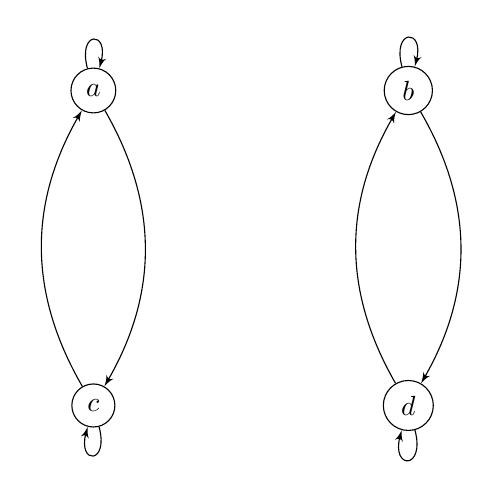
\begin{tikzpicture}
            % Vertices
            \node[vertex] (a) at (0,0) {$a$};
            \node[vertex] (b) at (4,0) {$b$};
            \node[vertex] (c) at (0,-4) {$c$};
            \node[vertex] (d) at (4,-4) {$d$};

            % Edges
            % a
            \draw[edge] (a) to[loop above] (a);
            \draw[edge] (a) to[bend left] (c);

            % b 
            \draw[edge] (b) to[loop above] (b);
            \draw[edge] (b) to[bend left] (d);

            % c
            \draw[edge] (c) to[bend left] (a);
            \draw[edge] (c) to[loop below] (c);

            % d 
            \draw[edge] (d) to[bend left] (b);
            \draw[edge] (d) to[loop below] (d);
        \end{tikzpicture}
    \end{figure}}
    \question{
    A Lemma in the book states: {\em Let $A$ be a set with $n$ elements, and let $R$ be a relation on $A$. If there is a path of length at least one in $R$ from $a$ to $b$, then there is such a path with length not exceeding $n$. Moreover, when $a \neq b$, if there is a path of length at least one in R from a to b, then there is such a path with length not exceeding $n-1$}. The book proves for the case that $a=b$. Find the proof for the case that $a \neq b$.}
    
    \answer{
        \begin{proof}
            Suppose that there is a path of at least one in $R$ from $a$ to $b$. Let $m$ be the length of the shortest path. Suppose that $x_0,x_1,x_2,\ldots,x_{m-1},x_m$, where $x_0=a$ and $x_m=b$, is such a path.
            \\[12pt]
            Suppose that $a\neq b$ and $m\geq n+1$. Since this path contains all $n$ vertices, by the pigeonhole principle, at least two are equal.
            \\[12pt]
            Suppose that $x_i=x_j$ with $0\leq i\leq j\leq m-1$. Then the path contains a circuit from $x_i$ to itself. This circuit can be deleted from the path from $a$ to $b$, leaving a path of shorter length. This process can be repeated until there are no more circuits, which means each vertex is contained in the path once and only once. Hence, the path contains exactly $n$ vertices, so there exists a path of length $n-1$.
        \end{proof}
    }
    \question{\label{question}
    Draw the directed graph that represents the relation: 
    \[ A \rel A=\{( a, a), ( a, b), ( b, c), ( c, b), ( c, d), ( d, a), ( d, b)\} \]
    where $A=\{a, b,c,d,e\}$}

    \answer{
    \begin{figure}[H]
        \centering
        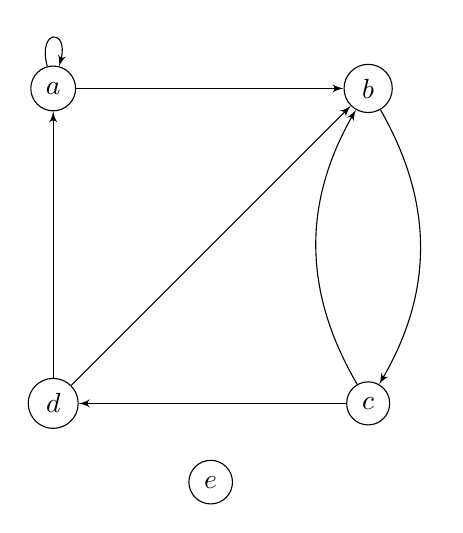
\begin{tikzpicture}
            % Vertices
            \node[vertex] (a) at (0,0) {$a$};
            \node[vertex] (b) at (4,0) {$b$};
            \node[vertex] (c) at (4,-4) {$c$};
            \node[vertex] (d) at (0,-4) {$d$};
            \node[vertex] (e) at (2,-5) {$e$};

            % Edges
            % a
            \draw[edge] (a) to[loop above] (a);
            \draw[edge] (a) to (b);
            
            % b
            \draw[edge] (b) to[bend left] (c);

            % c
            \draw[edge] (c) to[bend left] (b);
            \draw[edge] (c) to (d);

            % d
            \draw[edge] (d) to (a);
            \draw[edge] (d) to (b);
        \end{tikzpicture}
    \end{figure}}
    \question{
    Find the matrix of the relation of $A \rel A$  from \hyperref[question]{Question 6} above.}

    \answer{
    \[ R = \begin{bmatrix}
        1 & 1 & 0 & 0 & 0 \\
        0 & 0 & 1 & 0 & 0 \\
        0 & 1 & 0 & 1 & 0 \\
        1 & 1 & 0 & 0 & 0 \\
        0 & 0 & 0 & 0 & 0 \\
    \end{bmatrix} \]}
    \question{
    From the directed graph of  question \hyperref[question]{Question 6} above draw the digraph of $\bar{R}$ (the complement of $R$).}

    \answer{
    \begin{figure}[H]
        \centering
        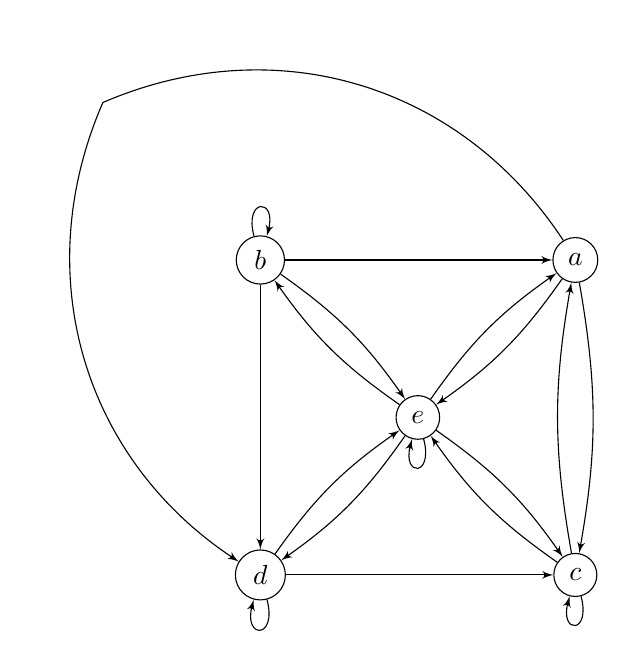
\begin{tikzpicture}
            % Vertices
            \node[vertex] (b) at (0,0) {$b$};
            \node[vertex] (c) at (4,-4) {$c$};
            \node[vertex] (d) at (0,-4) {$d$};
            \node[vertex] (a) at (4,0) {$a$};
            \node[vertex] (e) at (2,-2) {$e$};

            % Edges
            % a
            \draw[edge] (a) to[bend right=40] (-2, 2) to[bend right=40] (d);
            \draw[edge] (a) to[bend left=10] (c);
            \draw[edge] (a) to[bend left=10] (e);

            % b
            \draw[edge] (b) to (a);
            \draw[edge] (b) to[loop above] (b);
            \draw[edge] (b) to (d);
            \draw[edge] (b) to[bend left=10] (e);

            % c
            \draw[edge] (c) to[bend left=10] (a);
            \draw[edge] (c) to[loop below] (c);
            \draw[edge] (c) to[bend left=10] (e);

            % d
            \draw[edge] (d) to (c);
            \draw[edge] (d) to[loop below] (d);
            \draw[edge] (d) to[bend left=10] (e);

            % e
            \draw[edge] (e) to[bend left=10] (a);
            \draw[edge] (e) to[bend left=10] (b);
            \draw[edge] (e) to[bend left=10] (c);
            \draw[edge] (e) to[bend left=10] (d);
            \draw[edge] (e) to[loop below] (e);
        \end{tikzpicture}
    \end{figure}}
    \question{
    Find the matrix of the relation of $A{\bar R}A$  from question \hyperref[question]{Question 6} above.}

    \answer{
    The complement of $R$ is the matrix:
    \[ \overline{R} = \begin{bmatrix}
        0 & 0 & 1 & 1 & 1 \\
        1 & 1 & 0 & 1 & 1 \\
        1 & 0 & 1 & 0 & 1 \\
        0 & 0 & 1 & 1 & 1 \\
        1 & 1 & 1 & 1 & 1 \\
    \end{bmatrix} \]}

    \question{
    From the directed graph of question \hyperref[question]{Question 6} above draw the digraph of $R^{-1}$ (the inverse of $R$).}

    \answer{
    \begin{figure}[H]
        \centering
        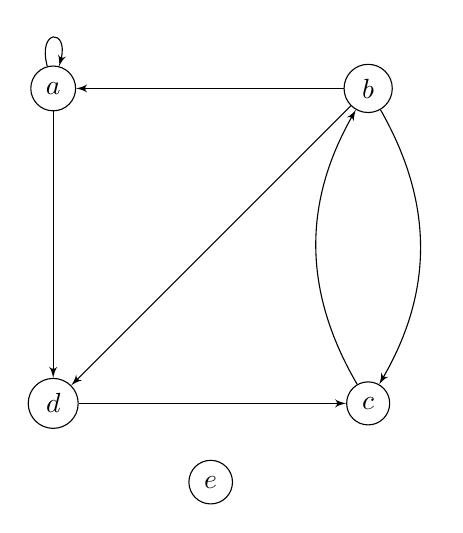
\begin{tikzpicture}
            % Vertices
            \node[vertex] (a) at (0,0) {$a$};
            \node[vertex] (b) at (4,0) {$b$};
            \node[vertex] (c) at (4,-4) {$c$};
            \node[vertex] (d) at (0,-4) {$d$};
            \node[vertex] (e) at (2,-5) {$e$};

            % Edges
            % a
            \draw[edge] (a) to[loop above] (a);
            \draw[edge] (a) to (d);

            % b
            \draw[edge] (b) to (a);
            \draw[edge] (b) to[bend left] (c);
            \draw[edge] (b) to (d);

            % c
            \draw[edge] (c) to[bend left] (b);

            % d
            \draw[edge] (d) to (c);

        \end{tikzpicture}
    \end{figure}}

    \question{
    Find the matrix of the relation of $A \rel^{-1}A$ from question \hyperref[question]{Question 6} above.}

    \answer{The inverse of $R$ is the matrix:
    \[ R^{-1} = \begin{bmatrix}
        1 & 0 & 0 & 1 & 0 \\
        1 & 0 & 1 & 1 & 0 \\
        0 & 1 & 0 & 0 & 0 \\
        0 & 0 & 1 & 0 & 0 \\
        0 & 0 & 0 & 0 & 0 \\
    \end{bmatrix} \]}

    \question{
    In $A \rel A$ from question \hyperref[question]{Question 6} above remove or add the least amount of elements so that $A \rel A$ represents an equivalence relation.}

    \answer{
    For $A \rel A$ to represent an equivalence relation, it must be reflexive, symmetric and transitive.    
    \\[12pt]
    To be reflexive, there must be a relation from each element to itself. Therefore, $(b,b),(c,c),(d,d),(e,e)$ must be added to $R$.
    \\[12pt]
    To be symmetric, $\forall x \forall y \in A ((x,y) \in R \leftrightarrow (y,x) \in R)$. Therefore, $(a,d)$ xor $(d,a)$ must change, $(b,d)$ xor $(d,b)$ must change and $(c,d)$ xor $(d,c)$ must change.
    \\[12pt]
    We can remove $(a,b), (c,d), (d,a), (d,b)$ to create a symmetric relation and add $(b,b),(c,c),(d,d),(e,e)$ to create a reflexive relation: $R = \set*{( a, a), (b, b), ( b, c), ( c, b), ( c, c), ( d, d), ( e, e)}$. As $\forall x \forall y \forall z \in A ((x,y) \in R \land (y,z) \in R \rightarrow (x,z) \in R)$,this is also a transitive relation. As this relation is reflexive, symmetric and transitive, it is an equivalence relation. Thus, with 8 changes we can transform $R$ into an equivalence relation.}
\end{document} 
